% v2-acmsmall-sample.tex, dated March 6 2012
% This is a sample file for ACM small trim journals
%
% Compilation using 'acmsmall.cls' - version 1.3 (March 2012), Aptara Inc.
% (c) 2010 Association for Computing Machinery (ACM)
%
% Questions/Suggestions/Feedback should be addressed to => "acmtexsupport@aptaracorp.com".
% Users can also go through the FAQs available on the journal's submission webpage.
%
% Steps to compile: latex, bibtex, latex latex
%
% For tracking purposes => this is v1.3 - March 2012

\documentclass[prodmode,acmtecs]{acmsmall} % Aptara syntax

% Package to generate and customize Algorithm as per ACM style
\usepackage[ruled]{algorithm2e}
\renewcommand{\algorithmcfname}{ALGORITHM}
\SetAlFnt{\small}
\SetAlCapFnt{\small}
\SetAlCapNameFnt{\small}
\SetAlCapHSkip{0pt}
\IncMargin{-\parindent}

% Metadata Information
\acmVolume{9}
\acmNumber{4}
\acmArticle{39}
\acmYear{2010}
\acmMonth{3}

% Copyright
%\setcopyright{acmcopyright}
%\setcopyright{acmlicensed}
%\setcopyright{rightsretained}
%\setcopyright{usgov}
%\setcopyright{usgovmixed}
%\setcopyright{cagov}
%\setcopyright{cagovmixed}

% DOI
\doi{0000001.0000001}

%ISSN
\issn{1234-56789}

% Document starts
\begin{document}

% Page heads
\markboth{G. Zhou et al.}{A Multifrequency MAC Specially Designed for WSN Applications}

% Title portion
\title{A Multifrequency MAC Specially Designed for Wireless Sensor Network Applications}
\author{GANG ZHOU
\affil{College of William and Mary}
YAFENG WU
\affil{University of Virginia}
TING YAN
\affil{Eaton Innovation Center}
TIAN HE
\affil{University of Minnesota}
CHENGDU HUANG
\affil{Google}
JOHN A. STANKOVIC
\affil{University of Virginia}
TAREK F. ABDELZAHER
\affil{University of Illinois at Urbana-Champaign}}
% NOTE! Affiliations placed here should be for the institution where the
%       BULK of the research was done. If the author has gone to a new
%       institution, before publication, the (above) affiliation should NOT be changed.
%       The authors 'current' address may be given in the "Author's addresses:" block (below).
%       So for example, Mr. Abdelzaher, the bulk of the research was done at UIUC, and he is
%       currently affiliated with NASA.

\begin{abstract}
Multifrequency media access control has been well understood in
general wireless ad hoc networks, while in wireless sensor networks,
researchers still focus on single frequency solutions. In wireless
sensor networks, each device is typically equipped with a single
radio transceiver and applications adopt much smaller packet sizes
compared to those in general wireless ad hoc networks. Hence, the
multifrequency MAC protocols proposed for general wireless ad hoc
networks are not suitable for wireless sensor network applications,
which we further demonstrate through our simulation experiments. In
this article, we propose MMSN, which takes advantage of
multifrequency availability while, at the same time, takes into
consideration the restrictions of wireless sensor networks. Through
extensive experiments, MMSN exhibits the prominent ability to utilize
parallel transmissions among neighboring nodes. When multiple physical
frequencies are available, it also achieves increased energy
efficiency, demonstrating the ability to work against radio
interference and the tolerance to a wide range of measured time
synchronization errors.
\end{abstract}


%
% The code below should be generated by the tool at
% http://dl.acm.org/ccs.cfm
% Please copy and paste the code instead of the example below. 
%
\begin{CCSXML}
<ccs2012>
 <concept>
  <concept_id>10010520.10010553.10010562</concept_id>
  <concept_desc>Computer systems organization~Embedded systems</concept_desc>
  <concept_significance>500</concept_significance>
 </concept>
 <concept>
  <concept_id>10010520.10010575.10010755</concept_id>
  <concept_desc>Computer systems organization~Redundancy</concept_desc>
  <concept_significance>300</concept_significance>
 </concept>
 <concept>
  <concept_id>10010520.10010553.10010554</concept_id>
  <concept_desc>Computer systems organization~Robotics</concept_desc>
  <concept_significance>100</concept_significance>
 </concept>
 <concept>
  <concept_id>10003033.10003083.10003095</concept_id>
  <concept_desc>Networks~Network reliability</concept_desc>
  <concept_significance>100</concept_significance>
 </concept>
</ccs2012>  
\end{CCSXML}

\ccsdesc[500]{Computer systems organization~Embedded systems}
\ccsdesc[300]{Computer systems organization~Redundancy}
\ccsdesc{Computer systems organization~Robotics}
\ccsdesc[100]{Networks~Network reliability}

%
% End generated code
%

% We no longer use \terms command
%\terms{Design, Algorithms, Performance}

\keywords{Wireless sensor networks, media access control,
multi-channel, radio interference, time synchronization}

\acmformat{Gang Zhou, Yafeng Wu, Ting Yan, Tian He, Chengdu Huang, John A. Stankovic,
and Tarek F. Abdelzaher, 2010. A multifrequency MAC specially
designed for  wireless sensor network applications.}
% At a minimum you need to supply the author names, year and a title.
% IMPORTANT:
% Full first names whenever they are known, surname last, followed by a period.
% In the case of two authors, 'and' is placed between them.
% In the case of three or more authors, the serial comma is used, that is, all author names
% except the last one but including the penultimate author's name are followed by a comma,
% and then 'and' is placed before the final author's name.
% If only first and middle initials are known, then each initial
% is followed by a period and they are separated by a space.
% The remaining information (journal title, volume, article number, date, etc.) is 'auto-generated'.

\begin{bottomstuff}
This work is supported by the National Science Foundation, under
grant CNS-0435060, grant CCR-0325197 and grant EN-CS-0329609.

Author's addresses: G. Zhou, Computer Science Department,
College of William and Mary; Y. Wu  {and} J. A. Stankovic,
Computer Science Department, University of Virginia; T. Yan,
Eaton Innovation Center; T. He, Computer Science Department,
University of Minnesota; C. Huang, Google; T. F. Abdelzaher,
(Current address) NASA Ames Research Center, Moffett Field, California 94035.
\end{bottomstuff}

\maketitle


\section{Introduction}

As a new technology, Wireless Sensor Networks (WSNs) has a wide
range of applications [Culler 2001,Bahl 2002,Akyildiz 2001], including
environment monitoring, smart buildings, medical care, industrial and
military applications. Among them, a recent trend is to develop
commercial sensor networks that require pervasive sensing of both
environment and human beings, for example, assisted living
[Akyildiz 2002,Harvard 2001,CROSSBOW] and smart homes
[Harvard 2001,Adya 2001,CROSSBOW].
% quote
\begin{quote}
``For these applications, sensor devices are incorporated into human
cloths [Natarajan 2001,Zhou 2006,Bahl 2002,Adya 2001] for monitoring
health related information like EKG readings, fall detection, and voice recognition".
\end{quote}
While collecting all these multimedia information
[Akyildiz 2002] requires a high network throughput, off-the-shelf
sensor devices only provide very limited bandwidth in a single
channel: 19.2Kbps in MICA2 [Bahl 2002] and 250Kbps in MICAz.

In this article, we propose MMSN, abbreviation for Multifrequency
Media access control for wireless Sensor Networks. The main
contributions of this work can be summarized as follows.
% itemize
\begin{itemize}
\item To the best of our knowledge, the MMSN protocol is the first
multifrequency MAC protocol especially designed for WSNs, in which
each device is equipped with a single radio transceiver and
the MAC layer packet size is very small.
\item Instead of using pairwise RTS/CTS frequency negotiation
[Adya 2001,Culler 2001; Tzamaloukas 2001; Zhou 2006],
we propose lightweight frequency assignments, which are good choices
for many deployed comparatively static WSNs.
\item We develop new toggle transmission and snooping techniques to
enable a single radio transceiver in a sensor device to achieve
scalable performance, avoiding the nonscalable ``one
control channel + multiple data channels'' design [Natarajan 2001].
\end{itemize}

% Head 1
\section{MMSN Protocol}

% Head 2
\subsection{Frequency Assignment}

We propose a suboptimal distribution to be used by each node, which is
easy to compute and does not depend on the number of competing
nodes. A natural candidate is an increasing geometric sequence, in
which
% Numbered Equation
\begin{equation}
\label{eqn:01}
P(t)=\frac{b^{\frac{t+1}{T+1}}-b^{\frac{t}{T+1}}}{b-1},
\end{equation}
where $t=0,{\ldots}\,,T$, and $b$ is a number greater than $1$.

In our algorithm, we use the suboptimal approach for simplicity and
generality. We need to make the distribution of the selected back-off
time slice at each node conform to what is shown in Equation
(\ref{eqn:01}). It is implemented as follows: First, a random
variable $\alpha$ with a uniform distribution within the interval
$(0, 1)$ is generated on each node, then time slice $i$ is selected
according to the following equation:
% Unnumbered Equation
\[
i=\lfloor(T+1)\log_b[\alpha(b-1)+1]\rfloor.
\]
It can be easily proven that the distribution of $i$ conforms to Equation
(\ref{eqn:01}).

So protocols [Bahl 2002,Culler 2001,Zhou 2006,Adya 2001,Culler 2001;
Tzamaloukas-01; Akyildiz-01] that use RTS/CTS
controls\footnote{RTS/CTS controls are required to be implemented by
802.11-compliant devices. They can be used as an optional mechanism
to avoid Hidden Terminal Problems in the 802.11 standard and
protocols based on those similar to [Akyildiz 2001] and
[Adya 2001].} for frequency negotiation and reservation are not
suitable for WSN applications, even though they exhibit good
performance in general wireless ad hoc
networks.

% Head 3
\subsubsection{Exclusive Frequency Assignment}

In exclusive frequency assignment, nodes first exchange their IDs
among two communication hops so that each node knows its two-hop
neighbors' IDs. In the second broadcast, each node beacons all
neighbors' IDs it has collected during the first broadcast period.

% Head 4
\paragraph{Eavesdropping}

Even though the even selection scheme leads to even sharing of
available frequencies among any two-hop neighborhood, it involves a
number of two-hop broadcasts. To reduce the communication cost, we
propose a lightweight eavesdropping scheme.

\subsection{Basic Notations}

As Algorithm~\ref{alg:one} states, for each frequency
number, each node calculates a random number (${\textit{Rnd}}_{\alpha}$) for
itself and a random number (${\textit{Rnd}}_{\beta}$) for each of its two-hop
neighbors with the same pseudorandom number generator.
% Algorithm
\begin{algorithm}[t]
\SetAlgoNoLine
\KwIn{Node $\alpha$'s ID ($ID_{\alpha}$), and node $\alpha$'s
neighbors' IDs within two communication hops.}
\KwOut{The frequency number ($FreNum_{\alpha}$) node $\alpha$ gets assigned.}
$index$ = 0; $FreNum_{\alpha}$ = -1\;
\Repeat{$FreNum_{\alpha} > -1$}{
        $Rnd_{\alpha}$ = Random($ID_{\alpha}$, $index$)\;
        $Found$ = $TRUE$\;
        \For{each node $\beta$ in $\alpha$'s two communication hops
    }{
      $Rnd_{\beta}$ = Random($ID_{\beta}$, $index$)\;
      \If{($Rnd_{\alpha} < Rnd_{\beta}$) \text{or} ($Rnd_{\alpha}$ ==
          $Rnd_{\beta}$ \text{and} $ID_{\alpha} < ID_{\beta}$)\;
      }{
        $Found$ = $FALSE$; break\;
      }
        }
     \eIf{$Found$}{
           $FreNum_{\alpha}$ = $index$\;
         }{
           $index$ ++\;
     }
      }
\caption{Frequency Number Computation}
\label{alg:one}
\end{algorithm}

Bus masters are divided into two disjoint sets, $\mathcal{M}_{RT}$
and $\mathcal{M}_{NRT}$.
% description
\begin{description}
\item[RT Masters]
$\mathcal{M}_{RT}=\{ \vec{m}_{1},\dots,\vec{m}_{n}\}$ denotes the
$n$ RT masters issuing real-time constrained requests. To model the
current request issued by an $\vec{m}_{i}$ in $\mathcal{M}_{RT}$,
three parameters---the recurrence time $(r_i)$, the service cycle
$(c_i)$, and the relative deadline $(d_i)$---are used, with their
relationships.
\item[NRT Masters]
$\mathcal{M}_{NRT}=\{ \vec{m}_{n+1},\dots,\vec{m}_{n+m}\}$ is a set
of $m$ masters issuing nonreal-time constrained requests. In our
model, each $\vec{m}_{j}$ in $\mathcal{M}_{NRT}$ needs only one
parameter, the service cycle, to model the current request it
issues.
\end{description}

Here, a question may arise, since each node has a global ID. Why
don't we just map nodes' IDs within two hops into a group of
frequency numbers and assign those numbers to all nodes within two
hops?

\section{Simulator}
\label{sec:sim}

If the model checker requests successors of a state which are not
created yet, the state space uses the simulator to create the
successors on-the-fly. To create successor states the simulator
conducts the following steps.
% enumerate
\begin{enumerate}
\item Load state into microcontroller model.
\item Determine assignments needed for resolving nondeterminism.
\item For each assignment.
      \begin{enumerate}
      \item either call interrupt handler or simulate effect of next instruction, or
      \item evaluate truth values of atomic propositions.
      \end{enumerate}
\item Return resulting states.
\end{enumerate}
Figure~\ref{fig:one} shows a typical microcontroller C program that
controls an automotive power window lift. The program is one of the
programs used in the case study described in Section~\ref{sec:sim}.
At first sight, the programs looks like an ANSI~C program. It
contains function calls, assignments, if clauses, and while loops.
% Figure
\begin{figure}
\centerline{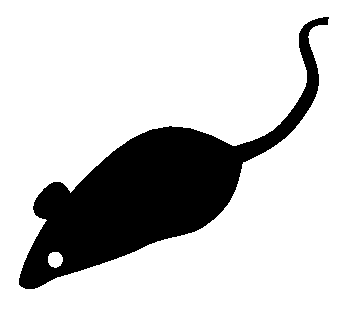
\includegraphics{acmsmall-mouse}}
\caption{Code before preprocessing.}
\label{fig:one}
\end{figure}

\subsection{Problem Formulation}

The objective of variable coalescence-based offset assignment is to find
both the coalescence scheme and the MWPC on the coalesced graph. We start
with a few definitions and lemmas for variable coalescence.

% Enunciations
\begin{definition}[Coalesced Node (C-Node)]A C-node is a set of
live ranges (webs) in the AG or IG that are coalesced. Nodes within the same
C-node cannot interfere with each other on the IG. Before any coalescing is
done, each live range is a C-node by itself.
\end{definition}

\begin{definition}[C-AG (Coalesced Access Graph)]The C-AG is the access
graph after node coalescence, which is composed of all C-nodes and C-edges.
\end{definition}

\begin{lemma}
The C-MWPC problem is NP-complete.
\end{lemma}
\begin{proof} C-MWPC can be easily reduced to the MWPC problem assuming a
coalescence graph without any edge or a fully connected interference graph.
Therefore, each C-node is an uncoalesced live range after value separation
and C-PC is equivalent to PC. A fully connected interference graph is made
possible when all live ranges interfere with each other. Thus, the C-MWPC
problem is NP-complete.
\end{proof}

\begin{lemma}[Lemma Subhead]The solution to the C-MWPC problem is no
worse than the solution to the MWPC.
\end{lemma}
\begin{proof}
Simply, any solution to the MWPC is also a solution to the
C-MWPC. But some solutions to C-MWPC may not apply to the MWPC (if any
coalescing were made).
\end{proof}

\section{Performance Evaluation}

During all the experiments, the Geographic Forwarding (GF)
[Akyildiz 2001] routing protocol is used. GF exploits geographic
information of nodes and conducts local data-forwarding to achieve
end-to-end routing. Our simulation is
configured according to the settings in
Table~\ref{tab:one}. Each run lasts for 2 minutes and
repeated 100 times. For each data value we present in the results,
we also give its 90\% confidence interval.
% Table
\begin{table}%
\tbl{Simulation Configuration\label{tab:one}}{%
\begin{tabular}{|l|l|}
\hline
TERRAIN{$^a$}   & (200m$\times$200m) Square\\\hline
Node Number     & 289\\\hline
Node Placement  & Uniform\\\hline
Application     & Many-to-Many/Gossip CBR Streams\\\hline
Payload Size    & 32 bytes\\\hline
Routing Layer   & GF\\\hline
MAC Layer       & CSMA/MMSN\\\hline
Radio Layer     & RADIO-ACCNOISE\\\hline
Radio Bandwidth & 250Kbps\\\hline
Radio Range     & 20m--45m\\\hline
\end{tabular}}
\begin{tabnote}%
\Note{Source:}{This is a table
sourcenote. This is a table sourcenote. This is a table
sourcenote.}
\vskip2pt
\Note{Note:}{This is a table footnote.}
\tabnoteentry{$^a$}{This is a table footnote. This is a
table footnote. This is a table footnote.}
\end{tabnote}%
\end{table}%

\section{Conclusions}

In this article, we develop the first multifrequency MAC protocol for
WSN applications in which each device adopts a
single radio transceiver. The different MAC design requirements for
WSNs and general wireless ad-hoc networks are
compared, and a complete WSN multifrequency MAC design (MMSN) is
put forth. During the MMSN design, we analyze and evaluate different
choices for frequency assignments and also discuss the nonuniform
back-off algorithms for the slotted media access design.

% Start of "Sample References" section

\section{Typical references in new ACM Reference Format}
A paginated journal article \cite{Abril07}, an enumerated
journal article \cite{Cohen07}, a reference to an entire issue \cite{JCohen96},
a monograph (whole book) \cite{Kosiur01}, a monograph/whole book in a series (see 2a in spec. document)
\cite{Harel79}, a divisible-book such as an anthology or compilation \cite{Editor00}
followed by the same example, however we only output the series if the volume number is given
\cite{Editor00a} (so Editor00a's series should NOT be present since it has no vol. no.),
a chapter in a divisible book \cite{Spector90}, a chapter in a divisible book
in a series \cite{Douglass98}, a multi-volume work as book \cite{Knuth97},
an article in a proceedings (of a conference, symposium, workshop for example)
(paginated proceedings article) \cite{Andler79}, a proceedings article
with all possible elements \cite{Smith10}, an example of an enumerated
proceedings article \cite{VanGundy07},
an informally published work \cite{Harel78}, a doctoral dissertation \cite{Clarkson85},
a master's thesis: \cite{anisi03}, an online document / world wide web resource \cite{Thornburg01}, \cite{Ablamowicz07},
\cite{Poker06}, a video game (Case 1) \cite{Obama08} and (Case 2) \cite{Novak03}
and \cite{Lee05} and (Case 3) a patent \cite{JoeScientist001},
work accepted for publication \cite{rous08}, 'YYYYb'-test for prolific author
\cite{SaeediMEJ10} and \cite{SaeediJETC10}. Other cites might contain
'duplicate' DOI and URLs (some SIAM articles) \cite{Kirschmer:2010:AEI:1958016.1958018}.
Boris / Barbara Beeton: multi-volume works as books
\cite{MR781536} and \cite{MR781537}.

% Appendix
\appendix
\section*{APPENDIX}
\setcounter{section}{1}
In this appendix, we measure
the channel switching time of Micaz [CROSSBOW] sensor devices.
In our experiments, one mote alternatingly switches between Channels
11 and 12. Every time after the node switches to a channel, it sends
out a packet immediately and then changes to a new channel as soon
as the transmission is finished. We measure the
number of packets the test mote can send in 10 seconds, denoted as
$N_{1}$. In contrast, we also measure the same value of the test
mote without switching channels, denoted as $N_{2}$. We calculate
the channel-switching time $s$ as
\begin{eqnarray}%
s=\frac{10}{N_{1}}-\frac{10}{N_{2}}. \nonumber
\end{eqnarray}%
By repeating the experiments 100 times, we get the average
channel-switching time of Micaz motes: 24.3$\mu$s.

\appendixhead{ZHOU}

% Acknowledgments
\begin{acks}
The authors would like to thank Dr. Maura Turolla of Telecom
Italia for providing specifications about the application scenario.
\end{acks}

% Bibliography
\bibliographystyle{ACM-Reference-Format-Journals}
\bibliography{acmsmall-sample-bibfile}
                             % Sample .bib file with references that match those in
                             % the 'Specifications Document (V1.5)' as well containing
                             % 'legacy' bibs and bibs with 'alternate codings'.
                             % Gerry Murray - March 2012

% History dates
\received{February 2007}{March 2009}{June 2009}

% Electronic Appendix
\elecappendix

\medskip

\section{This is an example of Appendix section head}

Channel-switching time is measured as the time length it takes for
motes to successfully switch from one channel to another. This
parameter impacts the maximum network throughput, because motes
cannot receive or send any packet during this period of time, and it
also affects the efficiency of toggle snooping in MMSN, where motes
need to sense through channels rapidly.

By repeating experiments 100 times, we get the average
channel-switching time of Micaz motes: 24.3 $\mu$s. We then conduct
the same experiments with different Micaz motes, as well as
experiments with the transmitter switching from Channel 11 to other
channels. In both scenarios, the channel-switching time does not have
obvious changes. (In our experiments, all values are in the range of
23.6 $\mu$s to 24.9 $\mu$s.)

\section{Appendix section head}

The primary consumer of energy in WSNs is idle listening. The key to
reduce idle listening is executing low duty-cycle on nodes. Two
primary approaches are considered in controlling duty-cycles in the
MAC layer.

\end{document}
% End of v2-acmsmall-sample.tex (March 2012) - Gerry Murray, ACM


